%%==================================================================
\section{Constructing the design}\label{sec:design}
%%==================================================================

The routine needs one row $\PP_{f,v}(T)$ per incidence. This section constructs
the rows and the matrices $C_{t,g}$, the partitions $S_{t,g}$ and the group
sequences $\sigma_f$ of Definition~\ref{def:design} from the scopes alone,
following \cite[Section 4]{OAI26}. The difficulty is to keep
$\deg\PP_{f,v}\le R$ with $R$ much smaller than $Q$: the degree of $H$ grows
linearly in $R$, and a small $R/Q$ reduces the number of Taylor coefficients
needed at each point. Rows chosen independently at the $Q$ points and
interpolated would in general have degree $Q$. The construction instead
produces, on a complete array of auxiliary coordinates, rows whose values at all
points are controlled together, and then places each incidence in a copy of that
array.

\subsection{Incidences and auxiliary coordinates}
Write $\mathcal I=\{(f,v):f\in\F,\ v\in I_f\}$, so $M=|\mathcal I|$, and let
$w$ and $b$ be as in \eqref{eq:M}. A factor with empty scope is a constant and is
assigned to group one at every point. If necessary adjoin a constant-one factor
with scope $\{v\}$ for every $v\in[n]$; this changes neither the product nor the
sum, and raises $b$ by at most one. With $b$ the bound after this step we assume
\begin{equation}\label{eq:nMb}
  n\ge1,\qquad b,w\ge1,\qquad n\le M\le bn .
\end{equation}
Throughout, $r\ge2$ and $1\le R<Q$ are integers and $0<\tau\le1/2$.

At each point $t$ the variable $x_v$ belongs to one group while a factor
containing it may be assigned to another. We shall choose
\[
  a_v\in[r]^{Q}\quad(v\in[n]),\qquad \delta_f\in[r]^{Q}\quad(f\in\F),
\]
where $a_v(t)$ is the group of $x_v$ and $\delta_f(t)$ the group of $f$ at the
point $t$, and the incidence $(f,v)$ will receive the label $(a_v,\delta_f)$.
Before choosing them, take all possible labels,
\begin{equation}\label{eq:B}
  \B=([r]^{Q})^2,\qquad u=(a_u,\delta_u),\qquad D=|\B|=r^{2Q}.
\end{equation}
An auxiliary vector $\zeta\in\Q^{\B}$ has one coordinate per label. For $t\in[Q]$
and $g\in[r]$ put
\begin{equation}\label{eq:SB}
  S^{\B}_{t,g}=\{u\in\B:a_u(t)=g\},
\end{equation}
which for fixed $t$ partition $\B$ into $r$ sets of size $D/r$. We seek, for each
$u\in\B$, a row $\PP_u(T)\in\Q[T]^{1\times\B}$ of degree at most $R-1$ with
$\PP_u(0)=\e_u$ such that the value $\ip{\PP_u(t)}{\zeta}$ is determined by
$\zeta|_{S^{\B}_{t,\delta_u(t)}}$ together with $C^{\B}\zeta$, where $C^{\B}$ is one
integer matrix with entries in $\{0,1,-1\}$ and few rows, the same for all $u$ and
$t$.

\subsection{The matrix $M_0$ and the measurements $C^{\B}$}
We seek $M_0\in\Q^{\B\times\B}$ that fixes $\ker C^{\B}$ and satisfies
\begin{equation}\label{eq:mismatch}
  M_0[u,y]\ne0\ \Longrightarrow\ \#\{s\in[Q]:a_y(s)\ne\delta_u(s)\}\le R-1 .
\end{equation}
The identity
\begin{equation}\label{eq:split}
  \zeta_u=\bigl((I-M_0)\zeta\bigr)_u+\sum_{y\in\B}M_0[u,y]\zeta_y
\end{equation}
explains both requirements: the first term is determined by $C^{\B}\zeta$ and
will be left independent of $T$, and each term of the sum will be multiplied by a
polynomial equal to one at zero and vanishing at every $t$ with
$a_y(t)\ne\delta_u(t)$, which \eqref{eq:mismatch} allows with degree at most
$R-1$.

For $s\in[Q]$ let $\vartheta_s:\B\to\B$ exchange the entries $a_u(s)$ and
$\delta_u(s)$ and leave the rest unchanged, and let $\Pi_s$ be its permutation
matrix, $(\Pi_s\zeta)_u=\zeta_{\vartheta_s(u)}$. The $\Pi_s$ commute and
$\Pi_s^2=I$. Put
\begin{equation}\label{eq:V0W0}
  V_0=\prod_{s=1}^{Q}\Pi_s,\qquad W_0=\frac12\sum_{s=1}^{Q}(I-\Pi_s).
\end{equation}
$V_0$ exchanges the two full sequences, so $V_0[u,y]\ne0$ forces $a_y=\delta_u$.
On a common eigenvector $\psi$ of the $\Pi_s$ with $\Pi_s\psi=-\psi$ for exactly
$j$ indices $s$,
\begin{equation}\label{eq:eigen}
  W_0\psi=j\psi,\qquad V_0\psi=(-1)^j\psi,\qquad V_0\,p(W_0)\psi=(-1)^jp(j)\psi
\end{equation}
for every polynomial $p$; so $V_0p(W_0)$ fixes $\psi$ whenever $p(j)=(-1)^j$.
For an interval $\mathcal J=\{A_0,\dots,A_0+R-1\}\subseteq\{0,\dots,Q\}$ the
polynomial
\begin{equation}\label{eq:fI}
  f_{\mathcal J}(z)=(-1)^{A_0}\sum_{j=0}^{R-1}(-2)^j\binom{z-A_0}{j},\qquad
  \binom{z-A_0}{j}=\frac1{j!}\prod_{a=0}^{j-1}(z-A_0-a),
\end{equation}
has degree at most $R-1$ and satisfies $f_{\mathcal J}(A_0+i)=(-1)^{A_0}(1-2)^i=(-1)^{A_0+i}$
for $0\le i<R$ by the binomial theorem. Set
\begin{equation}\label{eq:M0}
  M_0=V_0\,f_{\mathcal J}(W_0).
\end{equation}

\begin{lemma}\label{lem:CB}
There is a matrix $C^{\B}\in\{0,1,-1\}^{c^{\B}\times\B}$ with
$c^{\B}\le D\Pr[\mathsf W\notin\mathcal J]$, where $\mathsf W\sim\Bin(Q,\frac{r-1}{2r})$,
such that $M_0\xi=\xi$ for every $\xi\in\ker C^{\B}$.\footnote{Lemma 4.1 of
\cite{OAI26}.}
\end{lemma}

\begin{proof}
For $(\alpha,\beta)\in[r]^2$ let $e_{\alpha\beta}$ be the indicator function of
that ordered pair. Exchanging the two entries of a pair has the orthogonal
eigenbasis
\[
  e_{\alpha\alpha}\ (\alpha\in[r]),\qquad e_{\alpha\beta}+e_{\beta\alpha},\qquad
  e_{\alpha\beta}-e_{\beta\alpha}\quad(1\le\alpha<\beta\le r),
\]
with eigenvalue $+1$ for the first two kinds and $-1$ for the third; there are
$r(r+1)/2$ vectors with eigenvalue $+1$ and $r(r-1)/2$ with $-1$. For each
$s\in[Q]$ choose one of these $r^2$ functions, $\psi_s:[r]^2\to\{0,1,-1\}$, and
put $\psi(u)=\prod_{s}\psi_s(a_u(s),\delta_u(s))$. The $D=r^{2Q}$ choices give
nonzero pairwise orthogonal vectors, since their inner products factor over $s$,
so they form a basis of $\Q^{\B}$ with entries in $\{0,1,-1\}$. If exactly $j$ of
the chosen $\psi_s$ have eigenvalue $-1$, then $W_0\psi=j\psi$ and
$V_0\psi=(-1)^j\psi$ by \eqref{eq:eigen}, so $M_0$ fixes $\psi$ whenever
$j\in\mathcal J$. Let the rows of $C^{\B}$ be the transposes of the basis vectors
with $j\notin\mathcal J$. A fraction $(r-1)/(2r)$ of the choices at each position
has eigenvalue $-1$, independently over the positions, so the fraction of basis
vectors retained is $\Pr[\mathsf W\notin\mathcal J]$. If $C^{\B}\xi=0$ then $\xi$
is orthogonal to the retained vectors, hence a combination of the others, all of
which $M_0$ fixes.
\end{proof}

For $\epsilon>0$ the condition
\begin{equation}\label{eq:tail}
  \Pr\Bigl[\Bin\Bigl(Q,\tfrac{r-1}{2r}\Bigr)\notin\mathcal J\Bigr]\le\epsilon
\end{equation}
gives $c^{\B}\le\epsilon D$; we shall use $\epsilon=\tau/(rb)$.

\begin{lemma}\label{lem:mismatch}
If $M_0[u,y]\ne0$ then $\#\{s\in[Q]:a_y(s)\ne\delta_u(s)\}\le R-1$.\footnote{Lemma
4.2 of \cite{OAI26}.}
\end{lemma}

\begin{proof}
Expand $f_{\mathcal J}(W_0)$ in the commuting matrices $\Pi_s$. Since
$\deg f_{\mathcal J}\le R-1$ and $\Pi_s^2=I$, each monomial is a scalar multiple
of $\prod_{s\in K}\Pi_s$ for some $K\subseteq[Q]$ with $|K|\le R-1$, and
$V_0\prod_{s\in K}\Pi_s=\prod_{s\notin K}\Pi_s$. A nonzero $(u,y)$ entry of this
permutation matrix requires $a_y(s)=\delta_u(s)$ for every $s\notin K$, leaving at
most $R-1$ positions where they may differ. If more than $R-1$ positions disagree,
every summand has zero $(u,y)$ entry.
\end{proof}

\subsection{The auxiliary rows}
For $M_0[u,y]\ne0$ put
\begin{equation}\label{eq:phi}
  E_{u,y}=\{s\in[Q]:a_y(s)\ne\delta_u(s)\},\qquad
  \varphi_{u,y}(T)=\prod_{s\in E_{u,y}}\Bigl(1-\frac Ts\Bigr),
\end{equation}
the empty product being one; then $\deg\varphi_{u,y}\le R-1$, $\varphi_{u,y}(0)=1$,
and $\varphi_{u,y}(t)=0$ whenever $a_y(t)\ne\delta_u(t)$. Define
\begin{equation}\label{eq:Pu}
  \PP_u(T)=\e_u^{\top}(I-M_0)+\sum_{\substack{y\in\B\\ M_0[u,y]\ne0}}M_0[u,y]\,\varphi_{u,y}(T)\,\e_y^{\top}.
\end{equation}

\begin{lemma}\label{lem:rows}
The rows \eqref{eq:Pu} have degree at most $R-1$ and $\PP_u(0)=\e_u^{\top}$. For
$t\in[Q]$ and $g\in[r]$ let $C^{\B}_{t,g}$ be the restriction of $C^{\B}$ to the
columns $S^{\B}_{t,g}$. For every $u$, $t$ and $g\ne\delta_u(t)$, and every
$\xi\in\Q^{S^{\B}_{t,g}}$,
\[
  C^{\B}_{t,g}\xi=0\ \Longrightarrow\ \ip{\PP_u(t)}{\tilde\xi}=0 .
\]
More generally, $\ip{\PP_u(t)}{\zeta}$ is determined by $\zeta|_{S^{\B}_{t,\delta_u(t)}}$
and $C^{\B}\zeta$.\footnote{Lemma 4.3 of \cite{OAI26}.}
\end{lemma}

\begin{proof}
The degree bound is that of the $\varphi_{u,y}$, and
$\PP_u(0)=\e_u^{\top}(I-M_0)+\e_u^{\top}M_0=\e_u^{\top}$. Applying
\eqref{eq:Pu} to $\zeta$,
\begin{equation}\label{eq:Puzeta}
  \ip{\PP_u(T)}{\zeta}=\bigl((I-M_0)\zeta\bigr)_u+\sum_{M_0[u,y]\ne0}M_0[u,y]\varphi_{u,y}(T)\zeta_y .
\end{equation}
At $T=t$ every summand with $a_y(t)\ne\delta_u(t)$ vanishes, so the remaining
summands involve only $y\in S^{\B}_{t,\delta_u(t)}$; if $\tilde\xi$ is supported on
$S^{\B}_{t,g}$ with $g\ne\delta_u(t)$ they are zero on $\tilde\xi$. The hypothesis
$C^{\B}_{t,g}\xi=0$ gives $C^{\B}\tilde\xi=0$, so $(I-M_0)\tilde\xi=0$ by
Lemma~\ref{lem:CB}. For the last assertion, two vectors with the same value of
$C^{\B}\zeta$ differ by an element of $\ker C^{\B}$, so $(I-M_0)\zeta$ is
determined by $C^{\B}\zeta$, and the other terms at $T=t$ use only
$\zeta|_{S^{\B}_{t,\delta_u(t)}}$.
\end{proof}

Fixing $t$ and writing $\zeta_g=\zeta|_{S^{\B}_{t,g}}$ we have
$C^{\B}\zeta=\sum_gC^{\B}_{t,g}\zeta_g$, so fixing each of the $r$ vectors
$C^{\B}_{t,g}\zeta_g$ fixes $C^{\B}\zeta$ while imposing separate conditions on
the $r$ auxiliary groups; then $\ip{\PP_u(t)}{\zeta}$ depends on
$\zeta|_{S^{\B}_{t,\delta_u(t)}}$ alone.

\subsection{Choosing the groups}
We now choose $(a_v)_v$ and $(\delta_f)_f$ and set $u_{f,v}=(a_v,\delta_f)$ for
$(f,v)\in\mathcal I$. A label $u$ occurring $c_u$ times needs $c_u$ positions in
distinct copies of the auxiliary array, so the number of copies is
\begin{equation}\label{eq:h}
  h=\max_{u\in\B}c_u,\qquad c_u=\#\{(f,v)\in\mathcal I:u_{f,v}=u\},
\end{equation}
and the actual variable groups $\{v:a_v(t)=g\}$ must be small.

\begin{lemma}\label{lem:labels}
Assume \eqref{eq:nMb}, let $D=r^{2Q}$ and suppose
\begin{equation}\label{eq:balance}
  2(b+w)D^2\le M,\qquad 2Qr^2\le n .
\end{equation}
One can choose $a_v,\delta_f\in[r]^{Q}$ deterministically, with
$\delta_f\equiv1$ for factors of empty scope, such that
\[
  \max_{u\in\B}\#\{(f,v)\in\mathcal I:(a_v,\delta_f)=u\}\le\frac{2M}D,\qquad
  \#\{v:a_v(t)=g\}\le\frac{2n}r\quad(t\in[Q],\ g\in[r]),
\]
in $\poly(n,M,|\F|,D,Q,r,b,w)$ bit operations.\footnote{Lemma 4.5 of \cite{OAI26}.}
\end{lemma}

\begin{proof}
First let all $a_v$, and all $\delta_f$ with nonempty $I_f$, be independent and
uniform on $[r]^{Q}$; then each label $u_{f,v}$ is uniform on $\B$. Put
$n_{t,g}=\#\{v:a_v(t)=g\}$ and
\[
  \Phi=\sum_{u\in\B}\Bigl(c_u-\frac MD\Bigr)^2,\qquad
  \Xi=\sum_{t=1}^{Q}\sum_{g=1}^{r}\Bigl(n_{t,g}-\frac nr\Bigr)^2 .
\]
Expanding the squares,
\[
  \Phi=\sum_{(f,v),(f',v')\in\mathcal I}\mathbf 1\{(a_v,\delta_f)=(a_{v'},\delta_{f'})\}-\frac{M^2}D,\qquad
  \Xi=\sum_{t=1}^{Q}\sum_{v,v'\in[n]}\mathbf 1\{a_v(t)=a_{v'}(t)\}-\frac{Qn^2}r .
\]
Two labels are independent unless they share a factor or a variable, and each
$(f,v)$ shares one with at most $b+w$ incidences including itself. Independent
pairs are equal with probability $1/D$, the others with probability at most one,
so $\mathbb E\Phi\le M(b+w)$. For $v\ne v'$ the values $a_v(t),a_{v'}(t)$ are
independent and uniform, so $\mathbb E\Xi=Qn(1-1/r)\le Qn$.

To fix the choices deterministically, fix the $a_v$ and the $\delta_f$ with
nonempty scope one at a time, each time choosing a value that does not increase
the conditional expectation of $\Phi/(M(b+w))+\Xi/(Qn)$; such a value exists
because the current expectation is the average over the possible values of the
next choice. The final value is at most two, and both summands are nonnegative, so
\[
  c_u\le\frac MD+\sqrt{2M(b+w)},\qquad n_{t,g}\le\frac nr+\sqrt{2Qn}.
\]
The inequalities \eqref{eq:balance} bound the square roots by $M/D$ and $n/r$.

For the cost, put $K=r^{Q}$, so $D=K^2$. Each indicator in $\Phi$ depends on at
most four of the choices $a_v,\delta_f,a_{v'},\delta_{f'}$, and each indicator in
$\Xi$ on at most two. After any partial fixing, the conditional probability of an
indicator is computed by enumerating at most $K^4=D^2$ values of the unfixed
choices it involves, and has denominator dividing $K^4$. Summing the $M^2+Qn^2$
indicators gives both expectations, with all rationals of
$O(\log(2D)+\log(2M)+\log(2n)+\log(2Q)+\log(2+b+w))$ bits. There are at most
$n+|\F|$ choices to fix, each with $K$ candidates.
\end{proof}

\subsection{Placing copies of the variables}
Assume \eqref{eq:balance} and apply Lemma~\ref{lem:labels}. Index $h$ copies of
the auxiliary array by $[h]\times\B$, and assign to each $(f,v)\in\mathcal I$ a
copy $c(f,v)\in[h]$ so that the positions $(c(f,v),u_{f,v})$ are distinct; this is
possible since no label occurs more than $h$ times, and
\begin{equation}\label{eq:hD}
  hD\le 2M\le 2bn .
\end{equation}
Define $\iota:\Q^n\to\Q^{[h]\times\B}$ by $(\iota x)_{c,u}=x_v$ if
$(c,u)=(c(f,v),u_{f,v})$ for some $(f,v)\in\mathcal I$, and $0$ otherwise; the
occupied positions are distinct, so this is well defined. Several positions may
contain the same $x_v$, and unused positions are zero. Let
$\pi_c:\Q^{[h]\times\B}\to\Q^{\B}$ be the projection onto the copy $c$. Put
\begin{equation}\label{eq:Pfv}
  \PP_{f,v}(T)=\PP_{u_{f,v}}(T)\,\pi_{c(f,v)}\,\iota,\qquad
  S_{t,g}=\{v:a_v(t)=g\},\qquad \sigma_f(t)=\delta_f(t).
\end{equation}
At $T=0$ the row $\PP_{f,v}$ extracts the content of position $(c(f,v),u_{f,v})$,
which is $x_v$; so $\PP_{f,v}(0)=\e_v^{\top}$, and its degree is at most $R-1$.
Lemma~\ref{lem:labels} gives $|S_{t,g}|\le 2n/r$. Define
\begin{equation}\label{eq:Ctg}
  \widetilde C=\diag(C^{\B},\dots,C^{\B})\ \ (h\text{ copies}),\qquad
  \widehat C=\widetilde C\iota,\qquad C_{t,g}=\widehat C|_{S_{t,g}},
\end{equation}
the restriction keeping the columns in $S_{t,g}$ and all rows. Thus
$\widehat Cx$ records the auxiliary measurements in every copy after the copies
have been filled from $x$. Each row of $\widetilde C$ has at most $D$ nonzero
entries, all $\pm1$; multiplication by $\iota$ adds entries lying in a common
column and discards unused positions, so every row of $C_{t,g}$ has sum of
absolute values at most $D$, and its value on a Boolean vector lies in
$[-D,D]\cap\Z$. If \eqref{eq:tail} holds, each $C_{t,g}$ has $hc^{\B}$ rows, and
\begin{equation}\label{eq:ctg}
  \sum_{g=1}^{r}c_{t,g}=rhc^{\B}\le rh\epsilon D\le 2r\epsilon M\le 2r\epsilon bn,
\end{equation}
which with $\epsilon=\tau/(rb)$ is at most $2\tau n$.

For the kernel condition fix $t$, $g\ne\sigma_f(t)$ and $(f,v)$, and let
$\xi\in\Q^{S_{t,g}}$ with $C_{t,g}\xi=0$. Then $\widetilde C\iota\tilde\xi=0$, so
$C^{\B}\pi_c\iota\tilde\xi=0$ for every copy $c$. Every nonzero coordinate of
$\pi_c\iota\tilde\xi$ contains a variable $v'$ with $a_{v'}(t)=g$, whose label has
first sequence $a_{v'}$, so this vector is supported on $S^{\B}_{t,g}$.
Lemma~\ref{lem:rows} in the copy $c(f,v)$, where $\delta_{u_{f,v}}(t)=\delta_f(t)=\sigma_f(t)\ne g$,
gives $\ip{\PP_{f,v}(t)}{\tilde\xi}=\ip{\PP_{u_{f,v}}(t)}{\pi_{c(f,v)}\iota\tilde\xi}=0$,
which is \eqref{eq:kernel}. All inputs of a factor use the group $\delta_f(t)$,
and the sum still ranges over exactly the $n$ Boolean variables.

\subsection{Coefficient bounds}
\begin{lemma}\label{lem:coeff}
Let $d_{\mathrm{den}}=(R-1)!\,Q!$. Then $d_{\mathrm{den}}\PP_u(T)\in\Z[T]^{1\times\B}$
for every $u$, and the sum of the absolute values of all coefficients of
$d_{\mathrm{den}}\PP_u(T)$ is $2^{O(Q\log Q)}$. The same holds for
$d_{\mathrm{den}}\PP_{f,v}(T)$. The matrices $M_0$, $C^{\B}$ and the rows can be
constructed in $\poly(D,Q,r)$ bit operations.\footnote{Lemma 4.6 of
\cite{OAI26}.}
\end{lemma}

\begin{proof}
For $0\le j<R$ the $j$th summand of $f_{\mathcal J}(W_0)$ is
\[
  (-1)^{A_0}(-2)^j\binom{W_0-A_0I}{j}=\frac{(-1)^{A_0+j}}{j!}\prod_{a=0}^{j-1}\bigl(2W_0-2(A_0+a)I\bigr),
\]
and each factor on the right is an integer matrix because
$2W_0=QI-\sum_s\Pi_s$. Since $j!$ divides $(R-1)!$ and $V_0$ is a permutation
matrix, $(R-1)!\,M_0$ is integral. The denominators of $\varphi_{u,y}$ divide
$\prod_{s\in E_{u,y}}s$, which divides $Q!$. This proves the common denominator.
With $\|A\|_\infty=\max_i\sum_j|A[i,j]|$ and $\|\sum_ja_jT^j\|_1=\sum_j|a_j|$,
we have $\|W_0\|_\infty\le Q$ and $0\le A_0+a\le Q$, so each factor
$2W_0-2(A_0+a)I$ has norm at most $4Q$, whence
\[
  \|M_0\|_\infty\le R(4Q)^{R-1},\qquad \|\varphi_{u,y}\|_1\le\prod_{s\in E_{u,y}}\Bigl(1+\frac1s\Bigr)\le 2^{Q}.
\]
The sum of absolute values of the coefficients in the row $d_{\mathrm{den}}\PP_u$
is at most $d_{\mathrm{den}}\bigl(1+(1+2^Q)R(4Q)^{R-1}\bigr)$, whose logarithm is
$O(Q\log Q)$ since $R<Q$. Passing to $\PP_{f,v}$ by \eqref{eq:Pfv} adds
coefficients in common columns and discards others, so the bound persists.
Enumerating the eigenbasis, forming $f_{\mathcal J}(W_0)$ and the $\varphi_{u,y}$
takes $\poly(D,Q,r)$ arithmetic operations on rationals of $O(Q\log Q)$ bits.
\end{proof}

\begin{lemma}[The completed design]\label{lem:complete}
Let $n,b,w\ge1$ and let $(I_f)_{f\in\F}$ be subsets of $[n]$ of size at most $w$
with each $v$ in at most $b$ of them, $M=\sum_f|I_f|$ and $n\le M\le bn$. Let
$r\ge2$, $1\le R<Q$, $0<\tau\le1/2$ and $D=r^{2Q}$ satisfy \eqref{eq:balance},
and let an interval $\mathcal J=\{A_0,\dots,A_0+R-1\}\subseteq\{0,\dots,Q\}$
satisfy
\begin{equation}\label{eq:tailreq}
  \Pr\Bigl[\Bin\Bigl(Q,\tfrac{r-1}{2r}\Bigr)\notin\mathcal J\Bigr]\le\frac{\tau}{rb}.
\end{equation}
Then all the data of Definition~\ref{def:design} can be constructed
deterministically with a number of bit operations polynomial in
$n$, $M$, $|\F|$, $D$, $Q$, $r$, $b$ and $w$.\footnote{Lemma 4.7
of \cite{OAI26}.}
\end{lemma}

\begin{proof}
Lemma~\ref{lem:CB} gives $C^{\B}$ with $c^{\B}\le\tau D/(rb)$; Lemmas
\ref{lem:mismatch} and \ref{lem:rows} give the auxiliary rows;
Lemma~\ref{lem:labels} gives the groups with $hD\le2M$ and $|S_{t,g}|\le 2n/r$.
The maps \eqref{eq:Pfv} and \eqref{eq:Ctg} give rows with $\PP_{f,v}(0)=\e_v^{\top}$,
degree at most $R-1\le R$, and the kernel condition; every row of $C_{t,g}$ has
absolute row sum at most $D$, and \eqref{eq:ctg} gives
$\sum_gc_{t,g}\le2\tau n$. Lemma~\ref{lem:coeff} gives \ref{D5}.
\end{proof}

\begin{figure}[t]
\centering
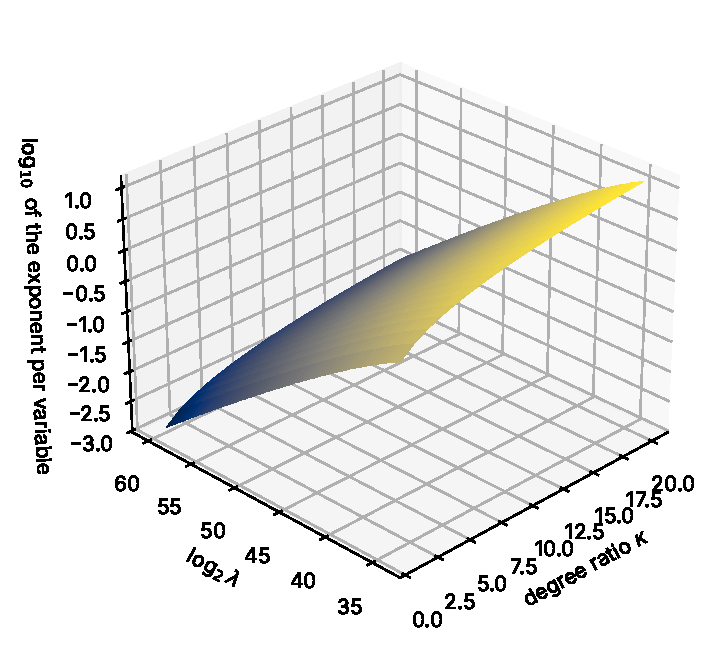
\includegraphics[width=0.78\textwidth]{figures/fig_costs}
\caption{The sum of the three costs of \eqref{eq:threecosts} per variable,
with the parameters \eqref{eq:params} for $\beta=2$, as a function of
$\lambda=\lceil\log n\rceil$ and of the degree ratio $\kappa$, drawn where the
hypotheses $r\ge2$ and $6R\le Q$ of Lemma~\ref{lem:params} hold. The surface
falls like $\nu^2/\sqrt\lambda$ in $\lambda$ and grows linearly in $\kappa$.}
\label{fig:costs}
\end{figure}

\subsection{Choosing the parameters}
The exponent of the routine depends on the three quantities of
\eqref{eq:threecosts}. The following choice bounds all three when $b$ and $w$
are bounded by a fixed power of $\log n$.

\begin{lemma}[Parameters]\label{lem:params}
Fix an integer $\beta\ge1$. Let $n\ge20$, $\lambda=\lceil\log n\rceil$,
$\nu=\lceil\log\lambda\rceil$, and suppose $b,w\le\lambda^{\beta}$ and
$n\le M\le bn$. For all sufficiently large $n$ the parameters
\begin{equation}\label{eq:params}
  r=\Bigl\lfloor\frac{\sqrt\lambda}{\nu^2}\Bigr\rfloor,\quad
  Q=\Bigl\lfloor\frac{\lambda}{128\nu}\Bigr\rfloor,\quad
  R=(\beta+3)\lceil\sqrt\lambda\rceil,\quad
  \tau=\frac1{r\lambda},\quad \epsilon=\frac1{br^2\lambda},\quad D=r^{2Q},
\end{equation}
with the interval $\mathcal J$ specified in the proof, satisfy the hypotheses of
Lemma~\ref{lem:complete}; moreover $R\ge32$, $6R\le Q$, $D\le2^{\lambda/128}$, and
\begin{equation}\label{eq:costs}
  \frac RQ\log\frac{2Q}R+\tau\log(2D+1)+\frac1r=O_\beta\Bigl(\frac{\nu^2}{\sqrt\lambda}\Bigr).
\end{equation}
Given $n,M,b,w$ the parameters can be computed and the hypotheses checked in
$\poly_\beta(\log n)$ bit operations, and for fixed $\beta$ only finitely many $n$
fail the checks.\footnote{Lemma 4.8 of \cite{OAI26}.}
\end{lemma}

\begin{proof}
For large $n$, $r=\Theta(\sqrt\lambda/\nu^2)$, $Q=\Theta(\lambda/\nu)$ and
$R=\Theta_\beta(\sqrt\lambda)$; so eventually $r\ge2$, $R\ge32$ and $6R\le Q$.
Since $\log r\le\nu/2$, $\log D=2Q\log r\le\lambda/128$. The balance inequalities
\eqref{eq:balance} hold for large $n$: $2(b+w)D^2\le4\lambda^\beta2^{\lambda/64}\le n\le M$
and $2Qr^2\le n$, because $Q,r$ are bounded by fixed powers of $\lambda$ while
$n>2^{\lambda-1}$. Put
\[
  \mu=\frac{Q(r-1)}{2r},\qquad A_0=\Bigl\lfloor\mu-\frac{R-1}2\Bigr\rfloor,\qquad
  \mathcal J=\{A_0,\dots,A_0+R-1\}.
\]
Then $Q/4\le\mu\le Q/2$, and since $R\le Q/6$ the interval lies in
$\{0,\dots,Q\}$; its centre is within one of $\mu$, and $R\ge32$ makes it contain
every integer within $R/4$ of $\mu$. For $\mathsf W\sim\Bin(Q,\frac{r-1}{2r})$,
Hoeffding's inequality \eqref{eq:hoeffding} with $s=R/4$ gives
\[
  \Pr[\mathsf W\notin\mathcal J]\le2e^{-R^2/(8Q)}\le2e^{-16(\beta+3)^2\nu}
  \le2^{-(\beta+2)\nu}\le\lambda^{-(\beta+2)}\le\frac1{br^2\lambda},
\]
using $R^2/(8Q)\ge(\beta+3)^2\lambda\cdot128\nu/(8\lambda)=16(\beta+3)^2\nu$,
$b\le\lambda^\beta$ and $r^2\le\lambda$. This is \eqref{eq:tailreq} with
$\epsilon=\tau/(rb)$, and $0<\tau\le1/2$ once $r\ge2$. Finally
$R/Q=O_\beta(\nu/\sqrt\lambda)$, $\log(2Q/R)=O(\nu)$ and
$\tau\log(2D+1)=O(1/r)$, while $1/r=O(\nu^2/\sqrt\lambda)$, which proves
\eqref{eq:costs}.

For the computation, $\lambda$ is the least integer with $n\le2^\lambda$ and $\nu$
the least with $\lambda\le2^\nu$; $r$ is the largest integer with
$r^2\nu^4\le\lambda$, $Q$ is an integer division, and $\lceil\sqrt\lambda\rceil$
comes from an integer square root. The algorithm reports failure if $r<2$ or
$Q\le R$; otherwise it forms $\tau,\epsilon,D$ and the endpoints of $\mathcal J$
in rational arithmetic and checks $\mathcal J\subseteq\{0,\dots,Q\}$,
\eqref{eq:balance}, $R\ge32$, $6R\le Q$, and \eqref{eq:tailreq}, whose left side
has denominator $(2r)^Q$ and is an exact rational computation. All of this takes
$\poly_\beta(\log n)$ bit operations, and the estimates above show that every check
passes for large $n$.
\end{proof}
